% !TEX root = ../dg.tex

\section{Tensor Algebras and Tensor Fields}

In order to give a more rigorous definition of differential forms (and in particular to get them to form a graded algebra), as well as more general tensor fields, we need to do some (multilinear) algebra and talk about tensor algebras and exterior algebras.

Before diving in, let me just give you my perspective on tensors. Basically, the point is that tensors are the right tool for turning multilinear algebra into linear algebra. More precisely, suppose we have three vector spaces $U$, $V$, and $W$, and a map $F: U \times V \to W$ which is multilinear (or, really, bilinear in this case). Again, this just means that $F$ is linear in each factor:
\[
	F(au_1 + bu_2, v) = aF(u_1,v) + b F(u_2,v) \qquad \text{and} \qquad F(u,cv_1 + dv_2) = cF(u,v_1) + dF(u,v_2).
\]

\begin{example}
	Any choice of inner product on $\R^n$ defines a bilinear map $\R^n \times \R^n \to \R$ by $(u,v) \mapsto \langle u, v \rangle$. Here $U = V = \R^n$ and $W = \R$.
\end{example}

\begin{example}
	Let $U = \R^n$, $V = \left(\R^n\right)^{n-1}$ and define a map $\R^n \times \left(\R^n\right)^{n-1} \cong \left(\R^n\right)^n \to \R$ by
	\[
		(u, (v_1, \dots , v_{n-1})) \mapsto \det \begin{bmatrix} u & v_1 & \dots & v_{n-1} \end{bmatrix}.
	\]
	This is also bilinear.
\end{example}

\begin{example}\label{ex:cross product as bilinear map}
	Let $U = V = W = \R^3$ and define the map $\R^3 \times \R^3 \to \R^3$ by $(u,v) \mapsto u \times v$, which is again bilinear.
\end{example}

Returning to the general setting, we have vector space $U$, $V$, and $W$ and a multilinear map $F: U \times V \to W$. Now suppose $w_0 \in W$ and we want to solve a problem of the form $F(u,v) = w_0$. Since $F$ is multilinear, you might hope that this is somehow just a linear algebra problem, which would be solvable, at least in principle. But, at least as stated, this is very much \emph{not} a linear problem…

\begin{example}\label{ex:cross product as bilinear map 2}
	Continuing with \cref{ex:cross product as bilinear map}, where $F \from \R^3 \times \R^3 \to \R^3$ is given by $F(u,v) = u \times v$, suppose we want to solve $F(u,v) = (x_0,y_0,z_0)$. Since $\R^3 \times \R^3 \cong \R^6$, we can think of $F$ as a map $\R^6 \to \R^3$ given by
	\[
		(u_1,u_2,u_3,v_1,v_2,v_3) \mapsto u \times v = (u_2 v_3 - u_3 v_2, u_3 v_1 - u_1 v_3, u_1 v_2 - u_2 v_1).
	\]
	So our problem is to solve
	\[
		(u_2 v_3 - u_3 v_2, u_3 v_1 - u_1 v_3, u_1 v_2 - u_2 v_1) = (x_0,y_0,z_0)
	\]
	for $(u_1,u_2,u_3,v_1,v_2,v_3)$, which is obviously a \emph{quadratic} system of equations, not a linear system.
\end{example}

To me\footnote{I want to emphasize here that this is just my perspective: I'm not claiming that everybody would agree with this characterization} the point of tensor products is to turn multilinear maps and problems into linear maps and problems.

\begin{definition}\label{def:tensor product}
	Given vector spaces $U$ and $V$, define the \emph{tensor product} $U \otimes V$ to be the vector space whose elements are of the form $u \times v$ for $u \in U$ and $v \in V$ so that 
	\begin{enumerate}
		\item $(u_1 + u_2) \otimes v = u_1 \otimes v + u_2 \otimes v$
		\item $u \otimes (v_1 + v_2) = u \otimes v_1 + u \otimes v_2$
		\item $a(u \otimes v) = (au) \otimes v = u \otimes (av)$
	\end{enumerate}
	for any $u,u_1,u_2 \in U$, $v,v_1,v_2 \in V$ and $a \in \R$.
\end{definition}

\begin{example}\label{ex:tensor product and outer product}
	If $U = \R^m$ and $V = \R^n$, then we can represent $u \otimes v$ by the $m \times n$ matrix 
	\[
		uv^T = \begin{bmatrix} u_1 \\ \vdots \\ u_m \end{bmatrix} \begin{bmatrix} v_1 & \dots & v_n \end{bmatrix} = \begin{bmatrix} u_i v_j \end{bmatrix}_{i,j}.
	\]
\end{example}

Here's the key theorem (or, if you start form a different perspective, the below theorem is the definition):

\begin{theorem}[Universal Property of the Tensor Product]\label{thm:tensor product universal property}
	If $\phi\from U \times V \to U \otimes V$ is the map given by $(u,v) \mapsto u \otimes v$ and $F \from U \times V \to W$ is bilinear, then there exists a unique \emph{linear} map $\widetilde{F} \from U \otimes V \to W$ making the following diagram commute:
	\begin{center}
	\begin{tikzcd}
		U \times V \arrow[r,"F"] \arrow[d,"\phi"'] & W \\
		U \otimes V \arrow[ur,"\widetilde{F}"',dashed]
	\end{tikzcd}
	\end{center}
	Moreover, this uniquely characterizes $U \otimes V$: any vector space satisfying this property must be isomorphic to $U \otimes V$.
\end{theorem}

\begin{example}
	Continuing \cref{ex:cross product as bilinear map,ex:cross product as bilinear map 2}, recall that $F\from \R^3 \times \R^3 \to \R^3$ is given by $F(u,v) = u \times v$, and \cref{thm:tensor product universal property} tells us there must be a linear map $\widetilde{F}\from \R^3 \otimes \R^3 \to \R^3$ so that
	\[
		(\widetilde{F} \circ \phi)(u,v) = F(u,v) = u \times v.
	\]
	Representing $u \otimes v$ by $u v^T$ as in \cref{ex:tensor product and outer product}, we see that $u \otimes v$ corresponds to the $3 \times 3$ matrix 
	\[
		\begin{bmatrix}  u_1 v_1 & u_1 v_2 & u_1 v_3 \\
 u_2 v_1 & u_2 v_2 & u_2 v_3 \\
 u_3 v_1 & u_3 v_2 & u_3 v_3 \end{bmatrix}.
	\]
	In general, $\R^3 \otimes \R^3 \cong \Mat_{3 \times 3}(\R) \cong \R^9$, so we can flatten this matrix to get a representation by a 9-dimensional vector, namely
	\[
		\begin{bmatrix}u_1 v_1 \\
 u_1 v_2 \\
 u_1 v_3 \\
 u_2 v_1 \\
 u_2 v_2 \\
 u_2 v_3 \\
 u_3 v_1 \\
 u_3 v_2 \\
 u_3 v_3\end{bmatrix}.
	\]
	So then $\widetilde{F}\from \R^9 \to \R^3$ is supposed to be linear, and hence must be represented by a $3 \times 9$ matrix $A$ so that
	\[
		A \begin{bmatrix}u_1 v_1 \\
 u_1 v_2 \\
 u_1 v_3 \\
 u_2 v_1 \\
 u_2 v_2 \\
 u_2 v_3 \\
 u_3 v_1 \\
 u_3 v_2 \\
 u_3 v_3\end{bmatrix}  = \begin{bmatrix} u_2 v_3 - u_3 v_2 \\ u_3 v_1 - u_1 v_3 \\ u_1 v_2 - u_2 v_1 \end{bmatrix}.
	\]
	Written out in this excruciating detail, it's now pretty obvious what $A$ has to be:
	\[
		A = \begin{bmatrix} 0 & 0 & 0 & 0 & 0 & 1 & 0 & -1 & 0 \\ 0 & 0 & -1 & 0 & 0 & 0 & 1 & 0 & 0 \\ 0 & 1 & 0 & -1 & 0 & 0 & 0 & 0 & 0 \end{bmatrix}.
	\]
\end{example}

\begin{proposition}\label{prop:tensor basis}
	If $u_1, \dots , u_m$ is a basis for $U$ and $v_1, \dots , v_n$ is a basis for $V$, then $\{e_i \otimes f_j\}_{i,j}$ is a basis for $U \otimes V$. In particular, $\dim U \otimes V = mn$.
\end{proposition}

\begin{notation}
	We will use $V^{\otimes k}$ to denote the $k$-fold tensor product of a vector space $V$ with itself; that is
	\[
		\underbrace{V \otimes \cdots \otimes V}_k = V \otimes (V \otimes \cdots \otimes (V \otimes V))
	\]
\end{notation}

\begin{definition}\label{def:tensor space}
	The \emph{tensor space of type $(r,s)$} associated with a vector space $V$ is the vector space
	\[
		V_r^s := V^{\otimes r} \otimes (V^\ast)^{\otimes s}.
	\]
	Elements of $V_r^s$ are called \emph{$(r,s)$-tensors}.
\end{definition}

\begin{example}
	An inner product $\langle \cdot , \cdot \rangle$ on $V$ is a symmetric $(0,2)$-tensor on $V$. Why? Well, $\langle \cdot , \cdot \rangle$ defines a bilinear map $V \times V \to \R$, and hence by \cref{thm:tensor product universal property} a (unique) linear map $V \otimes V \to \R$. In other words, an inner product determines an element of $(V \otimes V)^\ast \cong V^\ast \otimes V^\ast = V_0^2$.
	\begin{exercise}
		Prove that $(V \otimes V)^\ast \cong V^\ast \otimes V^\ast$
	\end{exercise}
\end{example}

\begin{example}
	A linear transformation $F\from V \to V$ (or, if you like, a square matrix) can be interpreted as a $(1,1)$-tensor. Why? $F$ induces a bilinear map $V^\ast \times V \to \R$ as follows: for $(\rho,v) \in V^\ast \times V$,
	\[
		(\rho, v ) \mapsto \rho(F(v)).
	\]
	Again, \cref{thm:tensor product universal property} implies that this bilinear map correponds to a linear map $V^\ast \otimes V \to \R$; that is, an element of the dual space $(V^\ast \otimes V)^\ast \cong V \otimes V^\ast = V_1^1$.
\end{example}

\begin{definition}\label{def:tensor algebra}
	The direct sum $\displaystyle \mathcal{T}(V):= \bigoplus_{r,s \geq 0} V_r^s$, where $V_0^0$ is the ground field of $V$, is called the \emph{tensor algebra} of $V$.
\end{definition}

\begin{remark}
	Terminology varies. Often \emph{tensor algebra} only refers to the algebra of $(\cdot , 0 )$-tensors, namely $\displaystyle \bigoplus_{r\geq 0} V_r^0 = \bigoplus_{r\geq 0} V^{\otimes r}$.
\end{remark}

In general, $\mathcal{T}(V)$ is noncommutative, associative, and (bi-)graded.

\begin{definition}\label{def:tensor bundle}
	The \emph{tensor bundle of type $(r,s)$} over a manifold $M$ is
	\[
		\mathcal{T}_r^s(M) := \bigsqcup_{p \in M} \left(T_pM\right)_r^s,
	\]
	which has a projection map $\pi\from \mathcal{T}_r^s(M) \to M$ sending a tensor based at a point to the point. 
	
\begin{exercise}
	If $M$ is an $n$-dimensional manifold, show that $\mathcal{T}_r^s(M)$ is a smooth manifold of dimension~$n^{r+s}$. 
\end{exercise}
	
	A \emph{tensor field} of type $(r,s)$ on $M$ is a smooth section of the tensor bundle $\mathcal{T}_r^s(M)$; i.e., a smooth map $\tau\from M \to \mathcal{T}_r^s(M)$ so that $\tau(p) \in \left(T_p M\right)_r^s$.
\end{definition}

\begin{example}
	A vector field on $M$ is (by definition) a $(1,0)$-tensor field on $M$.
\end{example}

\begin{example}
	A 1-form on $M$ is (again, by definition) a $(0,1)$-tensor field.
\end{example}

\begin{example}
	A Riemannian metric (which we've informally defined to be a smooth choice of inner product on each tangent space) is a (symmetric) $(0,2)$-tensor field on $M$. More precisely, we can define a \emph{Riemannian metric} on a manifold $M$ to be a smooth $(0,2)$-tensor field $g$ on $M$ so that, for each $p \in M$, $g_p = g(p)$ satisfies the axioms of an inner product on $T_p(M)$; that is, in addition to being bilinear (which is guaranteed by the fact it is a $(0,2)$-tensor), it must be symmetric ($g_p(u,v) = g_p(v,u)$) and positive-definite ($g_p(v,v) \geq 0$ with equality if and only if $v=0$).
	
	Note: when I write something like $g_p(u,v)$ I'm technically thinking of $g_p$ as the associated bilinear map $T_pM \times T_pM \to \R$, but in coordinates we also often use notation like $g = \sum_{i,j} g_{ij} dx_i \otimes dx_j$, which more closely matches up with the idea of $g$ being a $(0,2)$-tensor field.
\end{example}

\begin{example}
	Consider the Riemmannian metric $g = \frac{1}{y^2}(dx \otimes dx + dy \otimes dy)$ (also commonly written as $ds^2 = \frac{1}{y^2}(dx^2 + dy^2)$) on $H = \{(x,y) \in \R^2 : y > 0\}$.\footnote{In undergraduate differential geometry courses like MATH 474, the Riemannian metric is more often called the First Fundamental Form.} This is the Poincaré half-plane model of the hyperbolic plane. In general, we can compute the length of a curve $\gamma(t) = (\gamma_1(t),\gamma_2(t))$ by integrating the length of $\gamma'(t)$ along the curve. Since $\gamma'(t) \in T_{\gamma(t)}H$, its length is 
	\[
		\sqrt{g_{\gamma(t)}(\gamma'(t),\gamma'(t))} = \sqrt{\frac{\gamma'(t) \cdot \gamma'(t)}{\gamma_2(t)^2}} = \frac{\|\gamma'(t)\|_E}{\gamma_2(t)},
	\] 
	where $\cdot$ is the standard dot product on the plane and $\| \, \|_E$ is the Euclidean norm (I can just use $\gamma_2(t)$ in the denominator, rather than $|\gamma_2(t)|$, because the second coordinate is always positive in $H$).
	
	It will turn out that the geodesics in this metric are the vertical lines and semicircles centered at points on the $x$-axis; see \cref{fig:hyperbolicgeodesics}. Let's compute distances between points on these geodesics.
	
	\begin{figure}[htbp]
		\centering
			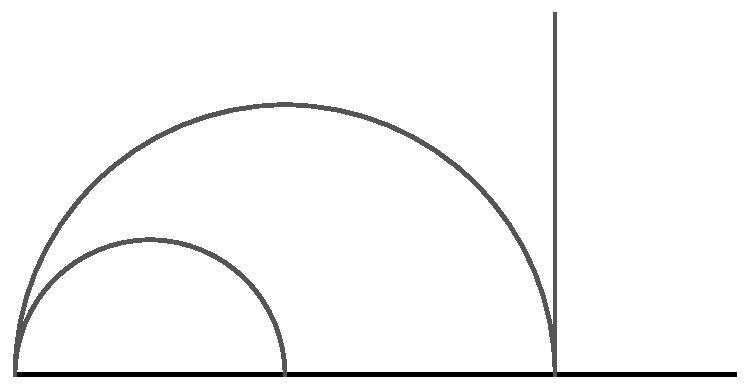
\includegraphics[height=1.5in]{hyperbolicgeodesics}
		\caption{Some geodesics in the Poincaré upper half-plane model of the hyperbolic plane.}
		\label{fig:hyperbolicgeodesics}
	\end{figure}
	
	For the vertical lines, we can parametrize the line through $(x_0,0)$ by $\gamma(t) = (x_0,t)$. So then $\gamma'(t) = (0,1)$ and the distance between $(x_0,y_0)$ and $(x_0,y_1)$ is
	\[
		\int_{y_0}^{y_1} \sqrt{g_{\gamma(t)}(\gamma'(t),\gamma'(t))}\,dt = \int_{y_0}^{y_1} \frac{1}{t}\, dt = \ln {y_1} - \ln {y_0} = \ln \left(\frac{y_1}{y_0}\right).
	\]
	Notice, in particular, that the $x$-axis is infinitely far away from any point in $H$.
	
	On the other hand, the semicircle of radius $r$ centered at $(x_0,0)$ can be parametrized by $\gamma(t) = (x_0 + r \cos t, r \sin t)$. Now $\gamma'(t) = r(-\sin t, \cos t)$, so the distance between $\gamma(\theta_0)$ and $\gamma(\theta_1)$ is
	\begin{multline*}
		\int_{\theta_0}^{\theta_1} \sqrt{g_{\gamma(t)}(\gamma'(t),\gamma'(t))}\, dt = \int_{\theta_0}^{\theta_1} \frac{r}{r \sin t} \, dt = \int_{\theta_0}^{\theta_1} \csc t\, dt = \operatorname{arctanh}(\cos\theta_0) - \operatorname{arctanh}(\cos \theta_1).
	\end{multline*}
\end{example}